%%%%%%%%%%%%%%%%%%%%%%%%%%%%%%%%%%%%%%%%%%%%%%%%%%%%%%%%%%%%%%%%%%%%%%%%%%%%%%%%%%%%%%%%%%%%%%%%%%%%%%%%%%%%%%%%%%%%%%%%%%%%%%%%%%%%%
% Preamble
%%%%%%%%%%%%%%%%%%%%%%%%%%%%%%%%%%%%%%%%%%%%%%%%%%%%%%%%%%%%%%%%%%%%%%%%%%%%%%%%%%%%%%%%%%%%%%%%%%%%%%%%%%%%%%%%%%%%%%%%%%%%%%%%%%%%%
%%%%%%%%%%%%%%%%%%%%%%%%%%%%%%%%%%%%%%%%%%%%%%%%%%%%%%%%%%%%%%%%%%%%%%%%%%%%%%%%%%%%%%%%%%%%%%%%%%%%%%%%%%%%%%%%%%%%%%%%%%%%%%%%%%%%%
% general packages & layout
\documentclass[a4paper,twoside,12pt]{book}
\usepackage{setspace}
\setstretch{1.25} % equals 1.5 line spacing in Word (base to base in LateX vs interline in Word)
\usepackage[nottoc]{tocbibind}
\usepackage{fancyhdr}
\usepackage[
% https://www.overleaf.com/learn/latex/Page_size_and_margins
% http://texdoc.net/texmf-dist/doc/latex/geometry/geometry.pdf
% total textwidth = 16-0.5-2x1.5 = 12.5cm
paperwidth=21cm,
paperheight=29.7cm,
bindingoffset=0cm, % space reserverd for binding
left=2.5cm, % left margin
right=2.5cm, % right margin
top=3cm, % top margin
bottom=2cm, % bottom margin
headheight=14pt
% CAVE! The result of these parameters depend on font size of header, etc. Check your final document for layout optimization
]{geometry} 
\setlength{\headsep}{10pt}  % distance between the baseline of the header and the top of the page text
\emergencystretch=1em  % avoid Overfull \hbox in references
\usepackage[titletoc]{appendix}


%%%%%%%%%%%%%%%%%%%%%%%%%%%%%%%%%%%%%%%%%%%%%%%%%%%%%%%%%%%%%%%%%%%%%%%%%%%%%%%%%%%%%%%%%%%%%%%%%%%%%%%%%%%%%%%%%%%%%%%%%%%%%%%%%%%%%
% adjust layout of lof and lot (separate per chapter, excluding chapters without figures or tables)
% cf. https://tex.stackexchange.com/questions/52746/include-chapters-in-list-of-figures-with-titletoc
\usepackage{etoolbox}
\makeatletter
% initial definitions of the chapter info (name and number)
\def\thischaptertitle{}\def\thischapternumber{}
\newtoggle{noFigs}
\newtoggle{noTables}
\apptocmd{\@chapter}%
{\gdef\thischaptertitle{#1}\gdef\thischapternumber{\thechapter}%
	\global\toggletrue{noFigs}
	\global\toggletrue{noTables}}{}{}
% the table/figure environment does the job: the first time it is used after a \chapter command, 
% it writes the information of the chapter to the LoF/LoT
\AtBeginDocument{%
	\AtBeginEnvironment{figure}{%
		\iftoggle{noFigs}{
			\addtocontents{lof}{\protect\contentsline {chapter}%
				{\protect\numberline {\thischapternumber}{\thischaptertitle}}{}{} }
			\global\togglefalse{noFigs}
		}{}
	}%
}
\AtBeginDocument{%
	\AtBeginEnvironment{table}{%
		\iftoggle{noTables}{
			\addtocontents{lot}{\protect\contentsline {chapter}%
				{\protect\numberline {\thischapternumber}{\thischaptertitle}}{}{} }
			\global\togglefalse{noTables}
		}{}
	}%
}
\makeatother


%%%%%%%%%%%%%%%%%%%%%%%%%%%%%%%%%%%%%%%%%%%%%%%%%%%%%%%%%%%%%%%%%%%%%%%%%%%%%%%%%%%%%%%%%%%%%%%%%%%%%%%%%%%%%%%%%%%%%%%%%%%%%%%%%%%%%
% bibliography
% options: maxbibnames: max number of author names in ref; mincitenames: min number of author names in citations
\usepackage[style=authoryear,backend=biber, maxbibnames=99, mincitenames=2, isbn=true, url=false]{biblatex}
% remove issn field from article references (but keep isbn for books)
\AtEveryBibitem{\clearfield{issn}}
\AtEveryCitekey{\clearfield{issn}}
% add bib files that contain references (this can go in 1 bib file or can be split up in several bib files)
% you can use http://git.macropus.org/citation-finder/ to convert Word references to bibtex
\addbibresource{./Bibliography/chap01.bib}
\addbibresource{./Bibliography/chap02.bib}
\addbibresource{./Bibliography/chap03.bib}
\addbibresource{./Bibliography/chap04.bib}
\addbibresource{./Bibliography/chap05.bib}
\addbibresource{./Bibliography/chap06.bib}
\addbibresource{./Bibliography/chap07.bib}
\addbibresource{./Bibliography/chap08.bib}
\addbibresource{./Bibliography/chap09.bib}
\addbibresource{./Bibliography/chap10.bib}


%%%%%%%%%%%%%%%%%%%%%%%%%%%%%%%%%%%%%%%%%%%%%%%%%%%%%%%%%%%%%%%%%%%%%%%%%%%%%%%%%%%%%%%%%%%%%%%%%%%%%%%%%%%%%%%%%%%%%%%%%%%%%%%%%%%%%
% graphics
\usepackage{graphicx}
\graphicspath{{./Graphs/}} % folder for graphs

%%%%%%%%%%%%%%%%%%%%%%%%%%%%%%%%%%%%%%%%%%%%%%%%%%%%%%%%%%%%%%%%%%%%%%%%%%%%%%%%%%%%%%%%%%%%%%%%%%%%%%%%%%%%%%%%%%%%%%%%%%%%%%%%%%%%%
% hyperlinks
\usepackage[hidelinks]{hyperref}
\usepackage[all]{hypcap} % go to the top of the reference instead of the caption

%%%%%%%%%%%%%%%%%%%%%%%%%%%%%%%%%%%%%%%%%%%%%%%%%%%%%%%%%%%%%%%%%%%%%%%%%%%%%%%%%%%%%%%%%%%%%%%%%%%%%%%%%%%%%%%%%%%%%%%%%%%%%%%%%%%%%
% acronyms (abbreviations)
\usepackage[toc,acronym,nomain]{glossaries}   % add nonumberlist as option to remove page numbers in list
\makeglossaries
\newacronym{mwm}{MWM}{Morris Water Maze}
\newacronym{rm}{RM-ANOVA}{Repeated measures ANOVA}
\newacronym{mmmmmm}{mm}{test2 mmmm}
\newacronym{rm2}{RM-ANOVA}{Repeated measures ANOVA}
\newacronym{rm3}{RM-ANOVA}{Repeated measures ANOVA}
\newacronym{orm}{ORM-ANOVA}{Repeated measures ANOVAaa}
	 % contains abbreviatons


%%%%%%%%%%%%%%%%%%%%%%%%%%%%%%%%%%%%%%%%%%%%%%%%%%%%%%%%%%%%%%%%%%%%%%%%%%%%%%%%%%%%%%%%%%%%%%%%%%%%%%%%%%%%%%%%%%%%%%%%%%%%%%%%%%%%%



%%%%%%%%%%%%%%%%%%%%%%%%%%%%%%%%%%%%%%%%%%%%%%%%%%%%%%%%%%%%%%%%%%%%%%%%%%%%%%%%%%%%%%%%%%%%%%%%%%%%%%%%%%%%%%%%%%%%%%%%%%%%%%%%%%%%%
% Start of document
%%%%%%%%%%%%%%%%%%%%%%%%%%%%%%%%%%%%%%%%%%%%%%%%%%%%%%%%%%%%%%%%%%%%%%%%%%%%%%%%%%%%%%%%%%%%%%%%%%%%%%%%%%%%%%%%%%%%%%%%%%%%%%%%%%%%%
\begin{document}
\pagenumbering{roman}
	
%%%%%%%%%%%%%%%%%%%%%%%%%%%%%%%%%%%%%%%%%%%%%%%%%%%%%%%%%%%%%%%%%%%%%%%%%%%%%%%%%%%%%%%%%%%%%%%%%%%%%%%%%%%%%%%%%%%%%%%%%%%%%%%%%%%%%
% title page
\pagestyle{empty} % no headers in this section
\begin{titlepage}
    \begin{center}
     
       
\includegraphics[width=5.5cm]{KUL_banner}%
       
       \vspace*{0.5cm}

        \textsc{Faculty of Psychology and}\\
        \textsc{Educational Sciences}\\ 
        KU LEUVEN\\
        
         \vspace*{0.7cm}

		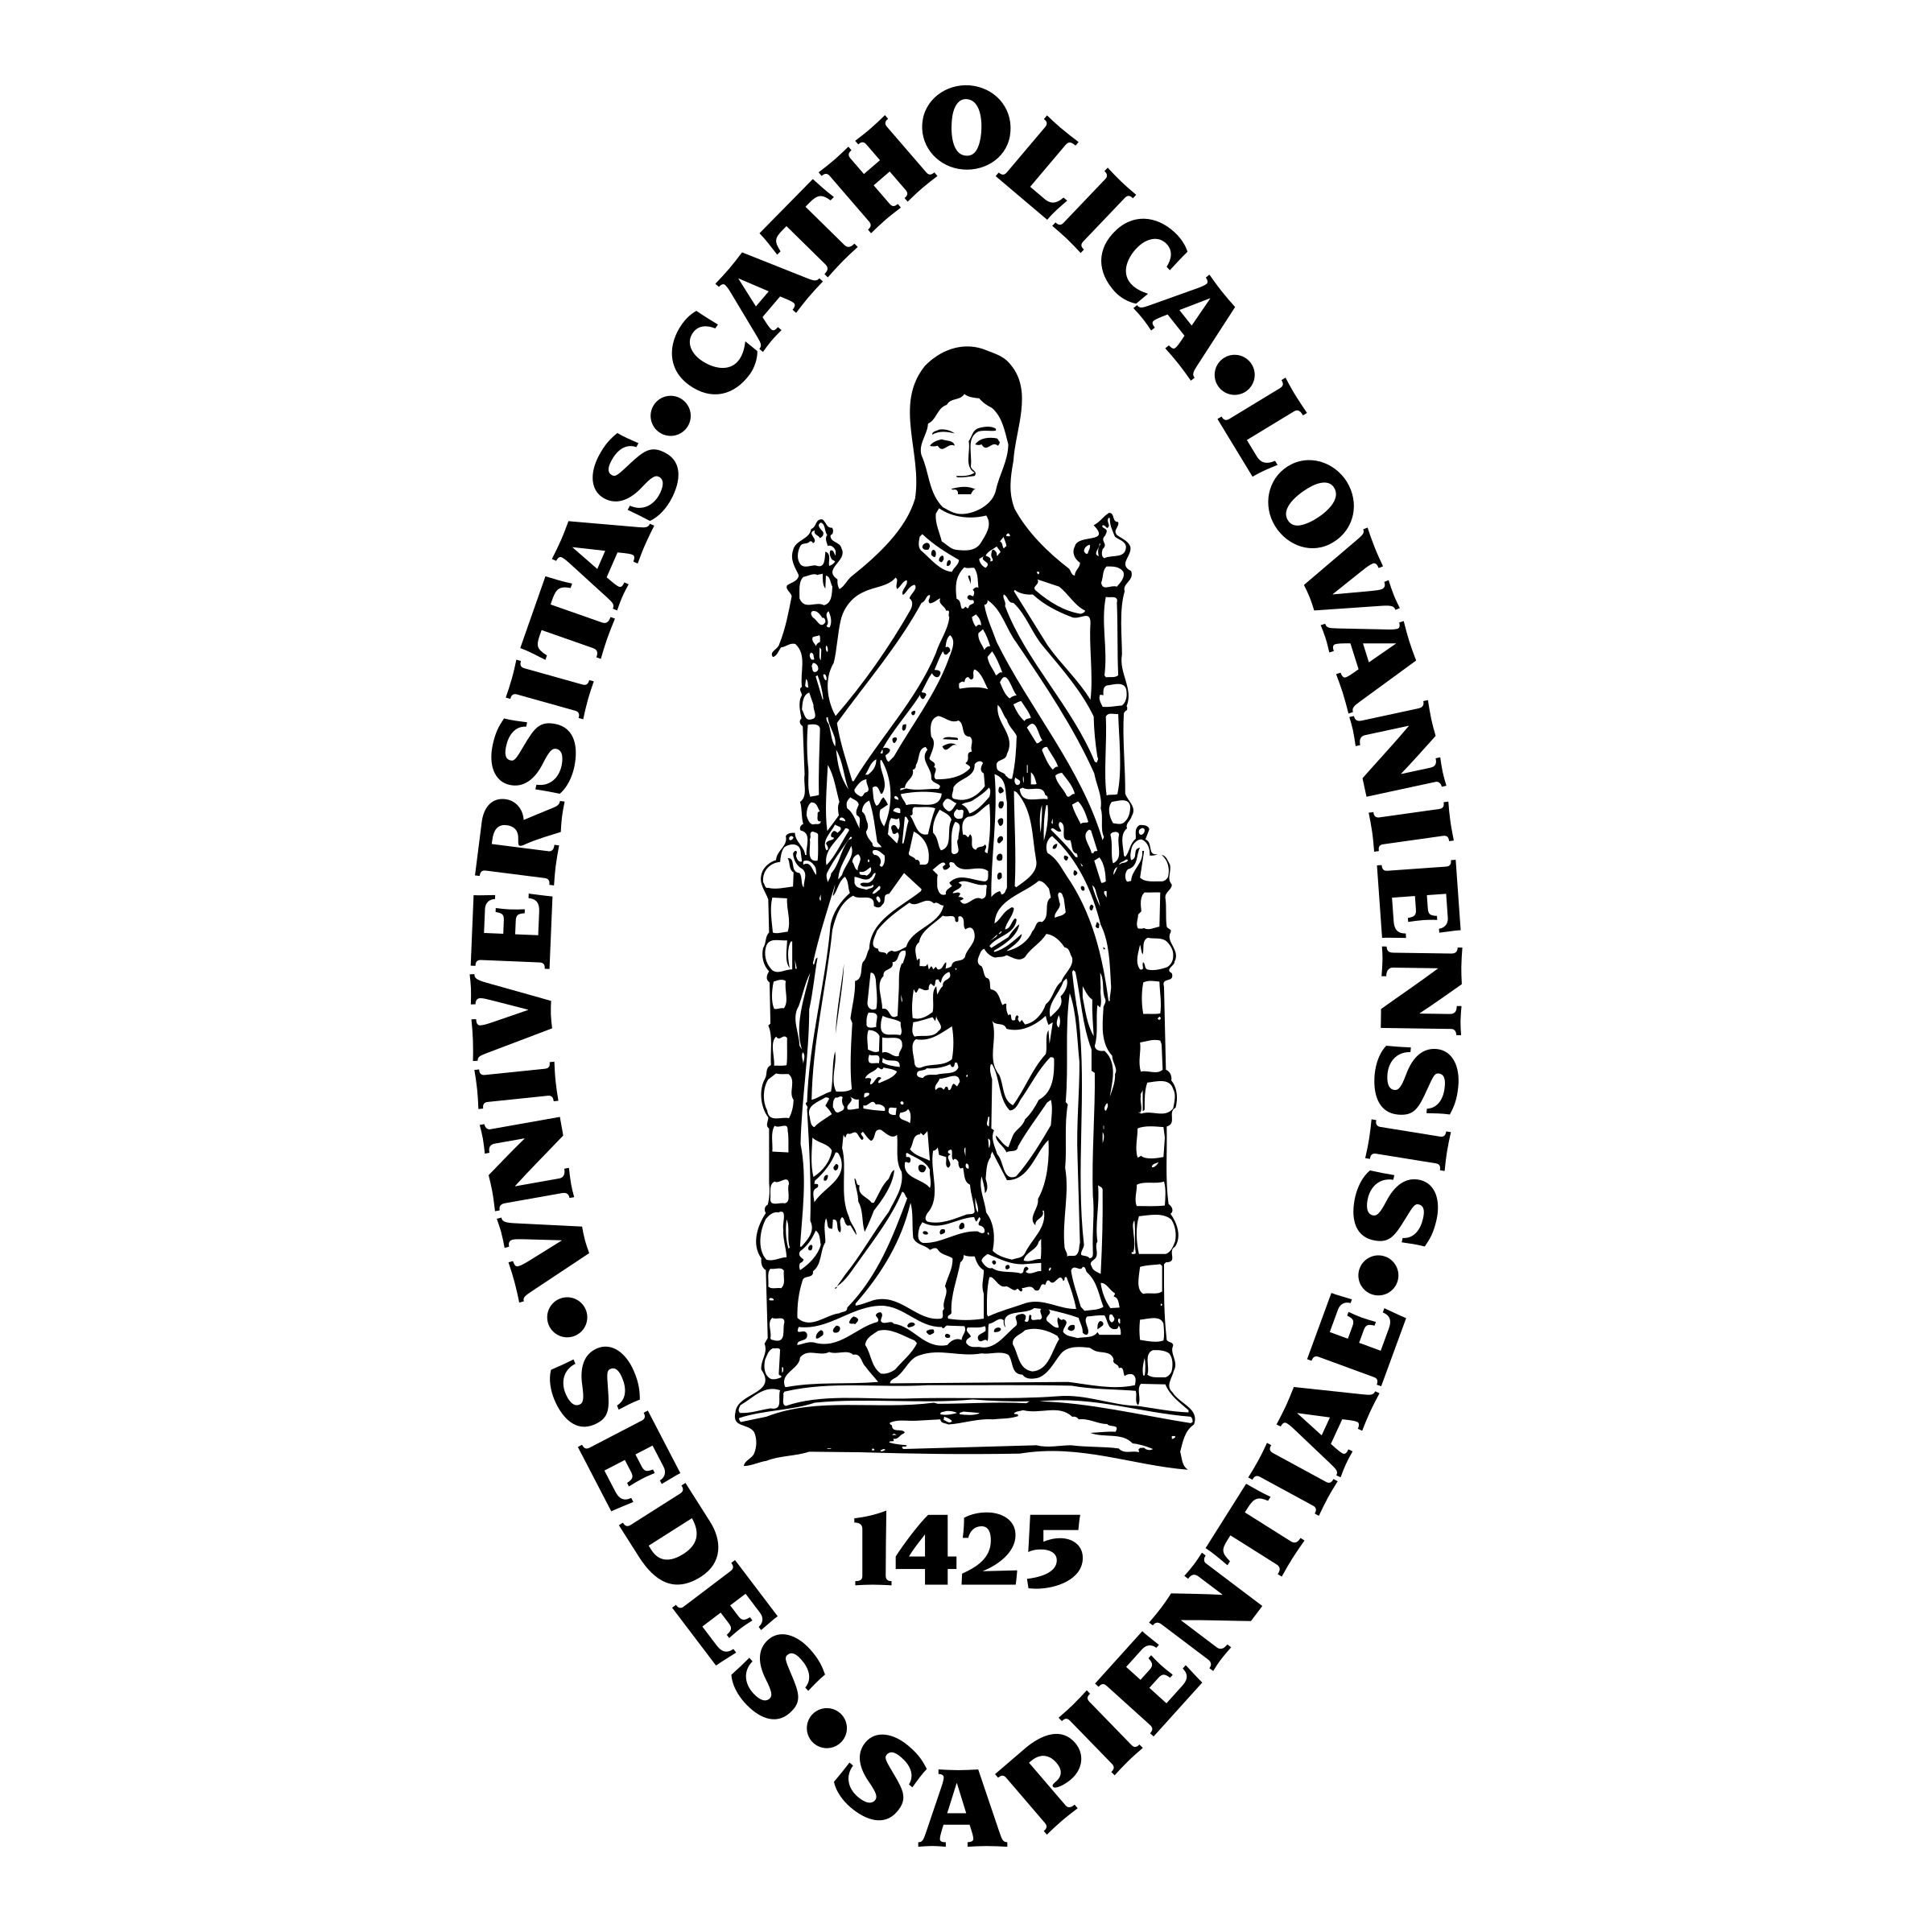
\includegraphics[height=1.8cm]{KUL_logo}
		
		 \vspace*{0.5cm}

 
        \Huge
        \textbf{Main Title}
 
        \vspace{0.5cm}
        \LARGE
        Subtitle
 
        \vspace{1.5cm}
 
        \textbf{Author}
 
        \vfill
 
        \vspace{0.8cm}
  
        \Large
        Supervisor: Prof. Dr. John Doe\\
        Co-supervisor: Dr. An Der\\[1\baselineskip]
      
        October, 2019\\[2\baselineskip]
        
                
        \large
        Dissertation to obtain the degree of Doctor of Psychology (PhD)\\
 
    \end{center}
\end{titlepage}
	


%%%%%%%%%%%%%%%%%%%%%%%%%%%%%%%%%%%%%%%%%%%%%%%%%%%%%%%%%%%%%%%%%%%%%%%%%%%%%%%%%%%%%%%%%%%%%%%%%%%%%%%%%%%%%%%%%%%%%%%%%%%%%%%%%%%%%
% frontmatter, contains acknowledgements, summary, samenvatting, list of figures, list of tables and abbreviatons, ...
% everything in this section will be ignored for numbering in TOC
\frontmatter
\pagestyle{plain} % no headers in this section but numbering in footer
\chapter[Acknowledgements]{Acknowledgements}
Text
\chapter[Summary]{Summary}
My summary
\chapter[Samenvatting]{Samenvatting}
Mijn samenvatting

\listoffigures
\listoftables
\printglossary[type=\acronymtype,title=List of Abbreviations,style=super]  % include list of abbreviations
\tableofcontents
\newpage
\pagestyle{empty}
\mbox{}


%%%%%%%%%%%%%%%%%%%%%%%%%%%%%%%%%%%%%%%%%%%%%%%%%%%%%%%%%%%%%%%%%%%%%%%%%%%%%%%%%%%%%%%%%%%%%%%%%%%%%%%%%%%%%%%%%%%%%%%%%%%%%%%%%%%%%
% mainmatter, contains all the chapters
\mainmatter
% headers, footers and lines
% https://www.overleaf.com/learn/latex/Headers_and_footers
\pagenumbering{arabic}
\pagestyle{fancy}
\fancyhf{} %  clear header and footer of standard style
\fancyfoot[CE,CO]{\thepage} % page number; L: left, R: right, C: center, E: even page, O: odd page
\fancyhead[LE]{\leftmark} % chapters short title
\fancyhead[RO]{\rightmark} % sections short title
%\fancyhead[LE,RO]{\leftmark} % chapters short title
%\fancyhead[RE,LO]{\rightmark} % sections short title
\renewcommand{\headrulewidth}{0pt} % head line
\renewcommand{\footrulewidth}{0pt} % foot line
% chapters
\begin{refsection} % refsection environment
\chapter[Short title]{Long title}

\section{Introduction}
Lorem ipsum dolor sit amet, consectetur adipiscing ...
We used the \acrfull{mwm} to test for spatial learning. However, with the \acrshort{mwm}, we... and \acrshort{mmmmmm} and \acrshort{rm}
\section{Methods}
Lorem ipsum dolor sit amet, consectetur adipiscing ... And \acrfull{rm} for... \acrfull{mmmmmm} and with \acrshort{mwm}
and \acrlong{mmmmmm} and \acrshort{rm2} and \acrshort{rm3} and \acrshort{orm}
\section{Results} 
And here we cite \cite{Famoye2015}. And also \citeauthor{Famoye2015}. 

The table \ref{table:1} is an example of referenced \LaTeX elements.

\begin{table}[h!]
	\centering
	\begin{tabular}{||c c c c||} 
		\hline
		Col1 & Col2 & Col2 & Col3 \\ [0.5ex] 
		\hline\hline
		1 & 6 & 87837 & 787 \\ 
		2 & 7 & 78 & 5415 \\
		3 & 545 & 778 & 7507 \\
		4 & 545 & 18744 & 7560 \\
		5 & 88 & 788 & 6344 \\ [1ex] 
		\hline
	\end{tabular}
	\caption{Table to test captions and labels}
	\label{table:1}
\end{table}

\begin{figure}[ht]
	\centering
	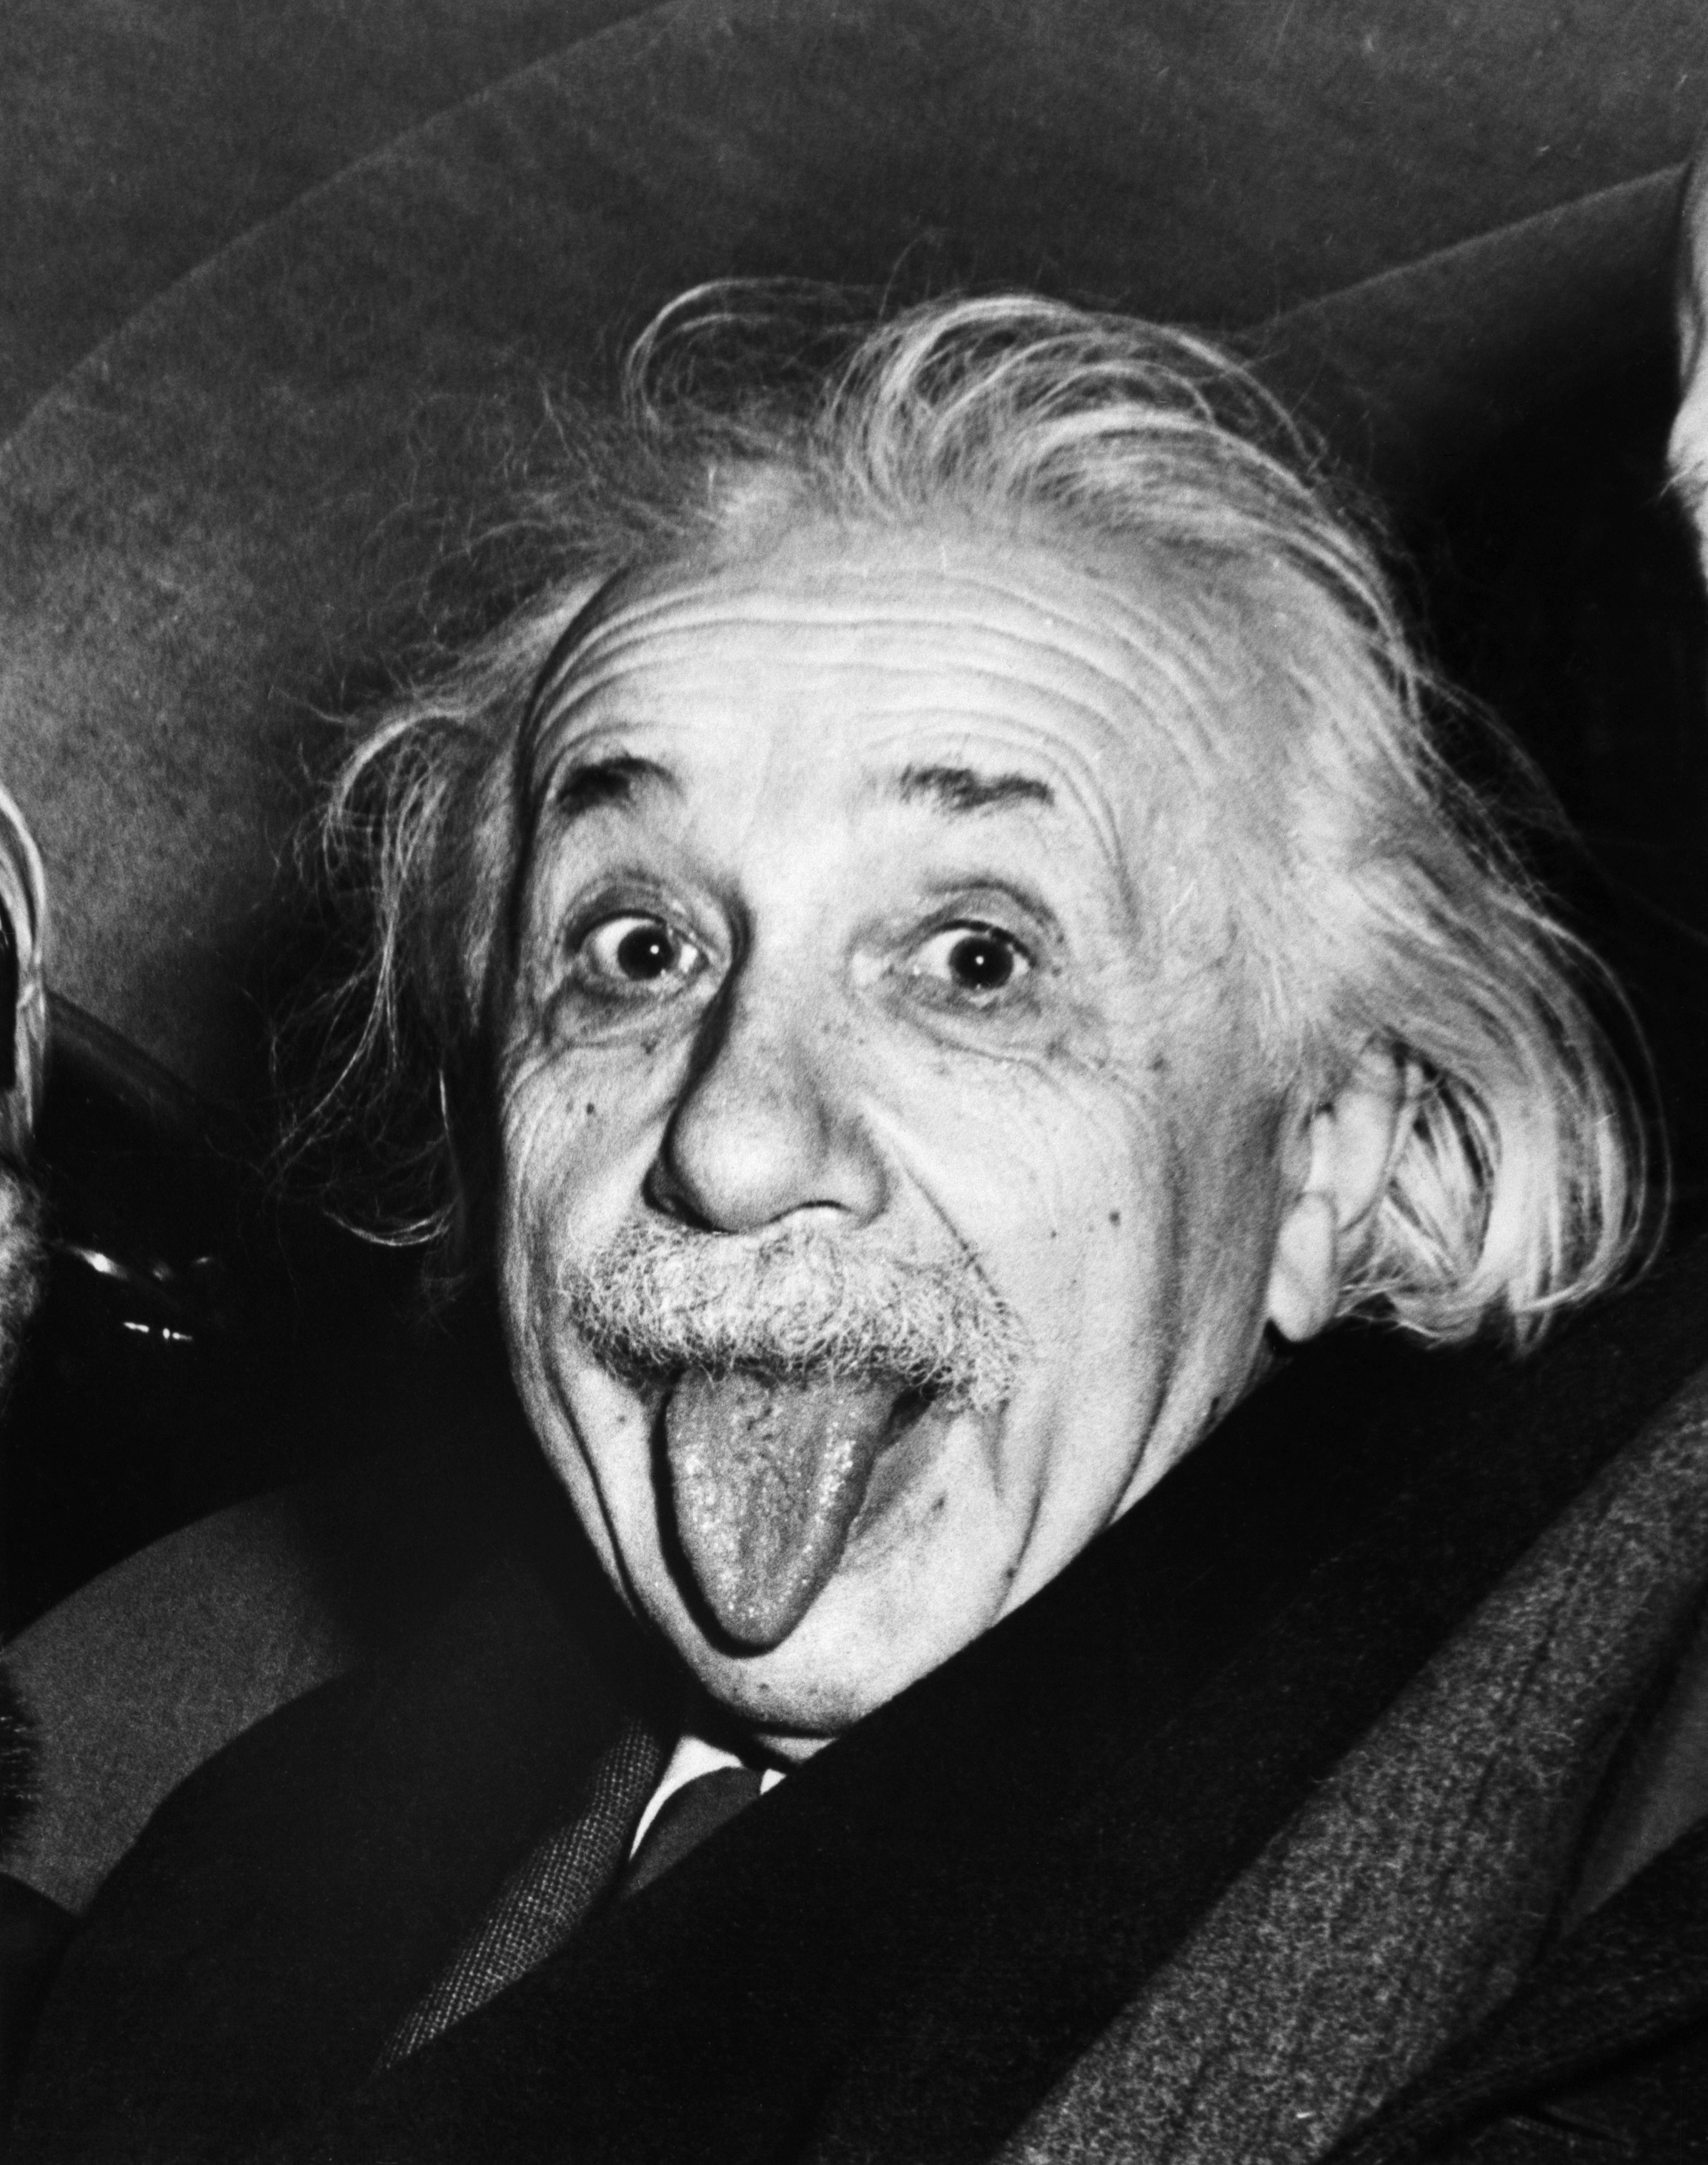
\includegraphics[width=\textwidth]{einstein.jpg}
	\caption[Einstein]{Einstein, a German-born theoretical physicist.}
	\centering
	\label{fig:1}
\end{figure}

As you can see in the photo \ref{fig:1}, ... Also, in page \pageref{fig:1}  we can see...

"But I must explain to you how all this mistaken idea of denouncing pleasure and praising pain was born and I will give you a complete account of the system, and expound the actual teachings of the great explorer of the truth, the master-builder of human happiness. No one rejects, dislikes, or avoids pleasure itself, because it is pleasure, but because those who do not know how to pursue pleasure rationally encounter consequences that are extremely painful. Nor again is there anyone who loves or pursues or desires to obtain pain of itself, because it is pain, but because occasionally circumstances occur in which toil and pain can procure him some great pleasure. To take a trivial example, which of us ever undertakes laborious physical exercise, except to obtain some advantage from it? But who has any right to find fault with a man who chooses to enjoy a pleasure that has no annoying consequences, or one who avoids a pain that produces no resultant pleasure?"

\subsection[SubShort]{Long title subsection}
This is a subsection
\subsubsection[SubSubShort]{Long title subsubsection}
This is a subsubsection
\paragraph{Paragraph title}
This is a paragraph
\subparagraph{Subparagraph title}
This is a subparagrah. "But I must explain to you how all this mistaken idea of denouncing pleasure and praising pain was born and I will give you a complete account of the system, and expound the actual teachings of the great explorer of the truth, the master-builder of human happiness. No one rejects, dislikes, or avoids pleasure itself, because it is pleasure, but because those who do not know how to pursue pleasure rationally encounter consequences that are extremely painful. Nor again is there anyone who loves or pursues or desires to obtain pain of itself, because it is pain, but because occasionally circumstances occur in which toil and pain can procure him some great pleasure. To take a trivial example, which of us ever undertakes laborious physical exercise, except to obtain some advantage from it? But who has any right to find fault with a man who chooses to enjoy a pleasure that has no annoying consequences, or one who avoids a pain that produces no resultant pleasure?"

"But I must explain to you how all this mistaken idea of denouncing pleasure and praising pain was born and I will give you a complete account of the system, and expound the actual teachings of the great explorer of the truth, the master-builder of human happiness. No one rejects, dislikes, or avoids pleasure itself, because it is pleasure, but because those who do not know how to pursue pleasure rationally encounter consequences that are extremely painful. Nor again is there anyone who loves or pursues or desires to obtain pain of itself, because it is pain, but because occasionally circumstances occur in which toil and pain can procure him some great pleasure. To take a trivial example, which of us ever undertakes laborious physical exercise, except to obtain some advantage from it? But who has any right to find fault with a man who chooses to enjoy a pleasure that has no annoying consequences, or one who avoids a pain that produces no resultant pleasure?"

"But I must explain to you how all this mistaken idea of denouncing pleasure and praising pain was born and I will give you a complete account of the system, and expound the actual teachings of the great explorer of the truth, the master-builder of human happiness. No one rejects, dislikes, or avoids pleasure itself, because it is pleasure, but because those who do not know how to pursue pleasure rationally encounter consequences that are extremely painful. Nor again is there anyone who loves or pursues or desires to obtain pain of itself, because it is pain, but because occasionally circumstances occur in which toil and pain can procure him some great pleasure. To take a trivial example, which of us ever undertakes laborious physical exercise, except to obtain some advantage from it? But who has any right to find fault with a man who chooses to enjoy a pleasure that has no annoying consequences, or one who avoids a pain that produces no resultant pleasure?"


\section{Discussion}

\addcontentsline{toc}{section}{References}
\printbibliography[heading=subbibliography, title={References}] % print section bibliography
\end{refsection}

\begin{refsection} % refsection environment
\chapter[Short title]{Long title}


\addcontentsline{toc}{section}{References}
\printbibliography[heading=subbibliography, title={References}] % print section bibliography

\begin{appendices}
	\chapter{Appendix I}
	This is a reference \cite{Al_Amin_1996}.
	
	This is a table. 
	
	\begin{table}[h!]
		\centering
		\begin{tabular}{||c c c c||} 
			\hline
			Col1 & Col2 & Col2 & Col3 \\ [0.5ex] 
			\hline\hline
			1 & 6 & 87837 & 787 \\ 
			2 & 7 & 78 & 5415 \\
			3 & 545 & 778 & 7507 \\
			4 & 545 & 18744 & 7560 \\
			5 & 88 & 788 & 6344 \\ [1ex] 
			\hline
		\end{tabular}
		\caption{Table to test captions and labels}
		\label{table:3}
	\end{table}

	This is a figure.
	
	\begin{figure}[ht]
		\centering
		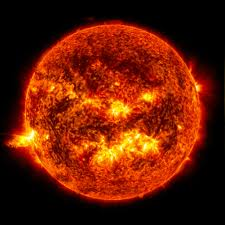
\includegraphics[]{sun.jpg}
		\caption[The sun]{The Sun is the star at the center of the Solar System.}
		\centering
		\label{fig:2}
	\end{figure}
	

	
	\chapter{Appendix II}
\end{appendices}

\end{refsection}

\begin{refsection} % refsection environment
\chapter[Short title]{Long title}

The table \ref{table:2} is an example of referenced \LaTeX elements.

\begin{table}[h!]
	\centering
	\begin{tabular}{||c c c c||} 
		\hline
		Col1 & Col2 & Col2 & Col3 \\ [0.5ex] 
		\hline\hline
		1 & 6 & 87837 & 787 \\ 
		2 & 7 & 78 & 5415 \\
		3 & 545 & 778 & 7507 \\
		4 & 545 & 18744 & 7560 \\
		5 & 88 & 788 & 6344 \\ [1ex] 
		\hline
	\end{tabular}
	\caption{Table to test captions and labels}
	\label{table:2}
\end{table}


\begin{figure}[ht]
	\centering
	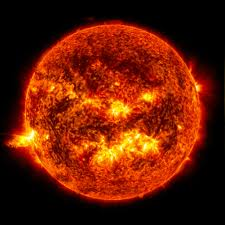
\includegraphics[]{sun.jpg}
	\caption[The sun]{The Sun is the star at the center of the Solar System.}
	\centering
	\label{fig:3}
\end{figure}

The sun(figure \ref{fig:3}), is a ... Also, on page \pageref{fig:3}  we can see...

And in \cite{Piiponniemi2017},...

\addcontentsline{toc}{section}{References}
\printbibliography[heading=subbibliography, title={References}] % print section bibliography
\end{refsection}

\begin{refsection} % refsection environment
\chapter[Short title]{Long title}

This is an acronym, MWM, for \acrfull{mwm}.

\addcontentsline{toc}{section}{References}
\printbibliography[heading=subbibliography, title={References}] % print section bibliography
\end{refsection}
\begin{refsection} % refsection environment
\chapter[Short title]{Long title}

\addcontentsline{toc}{section}{References}
\printbibliography[heading=subbibliography, title={References}] % print section bibliography
\end{refsection}
\begin{refsection} % refsection environment
\chapter[Short title]{Long title}

\addcontentsline{toc}{section}{References}
\printbibliography[heading=subbibliography, title={References}] % print section bibliography
\end{refsection}
\begin{refsection} % refsection environment
\chapter[Short title]{Long title}

\addcontentsline{toc}{section}{References}
\printbibliography[heading=subbibliography, title={References}] % print section bibliography
\end{refsection}
\begin{refsection} % refsection environment
\chapter[Short title]{Long title}

\addcontentsline{toc}{section}{References}
\printbibliography[heading=subbibliography, title={References}] % print section bibliography
\end{refsection}
\begin{refsection} % refsection environment
\chapter[Short title]{Long title}

\addcontentsline{toc}{section}{References}
\printbibliography[heading=subbibliography, title={References}] % print section bibliography
\end{refsection}
\begin{refsection} % refsection environment
\chapter[Short title]{Long title}

\addcontentsline{toc}{section}{References}
\printbibliography[heading=subbibliography, title={References}] % print section bibliography
\end{refsection}


%%%%%%%%%%%%%%%%%%%%%%%%%%%%%%%%%%%%%%%%%%%%%%%%%%%%%%%%%%%%%%%%%%%%%%%%%%%%%%%%%%%%%%%%%%%%%%%%%%%%%%%%%%%%%%%%%%%%%%%%%%%%%%%%%%%%%
% backmatter
% everything in this section will be ignored for numbering in TOC
\backmatter
\pagestyle{empty} % no headers in this section
\chapter[Curriculum Vitae]{Curriculum vitae}
Text


%%%%%%%%%%%%%%%%%%%%%%%%%%%%%%%%%%%%%%%%%%%%%%%%%%%%%%%%%%%%%%%%%%%%%%%%%%%%%%%%%%%%%%%%%%%%%%%%%%%%%%%%%%%%%%%%%%%%%%%%%%%%%%%%%%%%%
% End of document
%%%%%%%%%%%%%%%%%%%%%%%%%%%%%%%%%%%%%%%%%%%%%%%%%%%%%%%%%%%%%%%%%%%%%%%%%%%%%%%%%%%%%%%%%%%%%%%%%%%%%%%%%%%%%%%%%%%%%%%%%%%%%%%%%%%%%
\end{document}
%%%%%%%%%%%%%%%%%%%%%%%%%%%%%%%%%%%%%%%%%%%%%%%%%%%%%%%%%%%%%%%%%%%%%%%%%%%%%%%%%%%%%%%%%%%%%%%%%%%%%%%%%%%%%%%%%%%%%%%%%%%%%%%%%%%%%
